\section{Auswertung}
\label{sec:Auswertung}

\subsection{Temperaturverläufe}
Die während des Versuches gemessenen Temperaturen von Reservoir 1 und Reservoir 2 sind in dem Diagramm \ref{fig:Temperaturverlauf} dargestellt.
Die Temperatur in $\si{\kelvin}$ wurde gegenüber der Zeit in $\si{\second}$ aufgetragen.
\begin{figure}
  \centering
  \includegraphics[width=\textwidth]{build/plot_0.pdf}
  \caption{Temperaturverlauf der Messwerte}
  \label{fig:Temperaturverlauf}
\end{figure}
% \subsubsection{Ausgleichsfunktion}
\begin{figure}
  \centering
  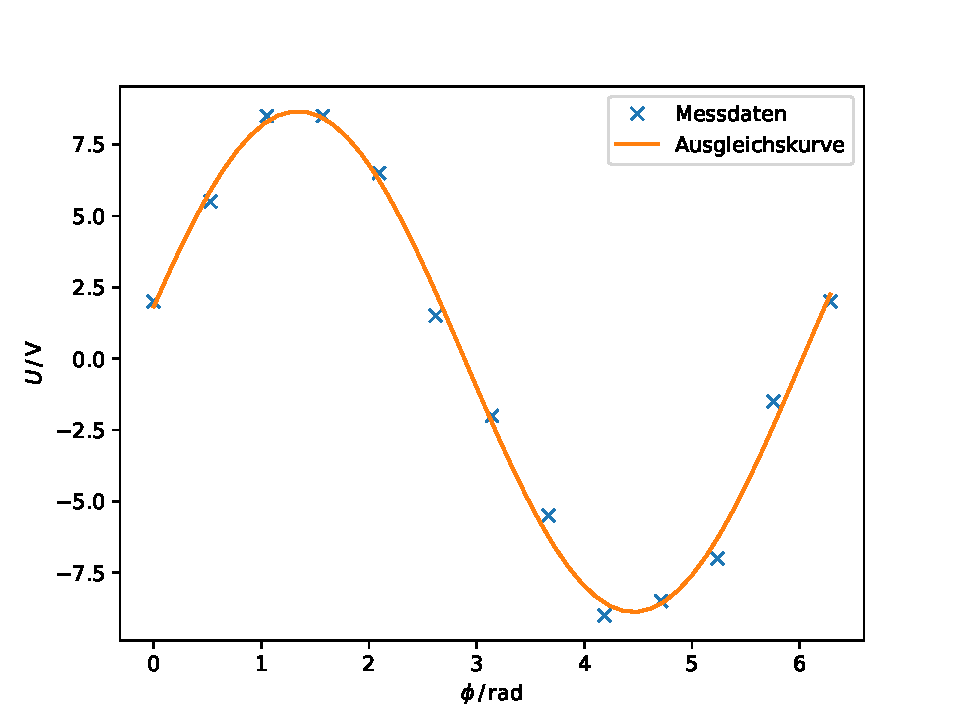
\includegraphics[width=\textwidth]{build/plot_1.pdf}
  \caption{Temperaturverlauf der Messwerte mit Ausgleichsfunktionen}
  \label{fig:Temperaturverlauf_Fit_1}
\end{figure}
Als erstes wird in \autoref{fig:Temperaturverlauf_Fit_1} der Temperaturverlauf durch die Funktion $T(t)=A\cdot t^2 + B\cdot t + C$ approximiert.
Daraus resultieren für die kalte Seite die Parameter $A=(1.9 \pm 1.7) \times 10^{-6} \frac{\si{\kelvin}}{\si{\second}^2}$, $B=(-0.0203 \pm 0.0017) \si{\kelvin\per\second}$ und $C=Q_{1,0}=294.15 \si{\kelvin}$ sowie
$A=(-3 \pm 8) \times 10^{-7} \frac{\si{\kelvin}}{\si{\second}^2}$, $B=(0.0240 \pm 0.0008) \si{\kelvin\per\second}$ und $C=Q_{2,0}=294.15 \si{\kelvin}$ für die warme Seite.


\subsection{Differentialquotient der nicht-linearen Ausgleichsrechnung}
Der Differentialquotient $\frac{\mathup{d}}{\mathup{d}t} T(t)$ der Ausgleichskurve ergibt sich aus:
\begin{align*}
  \frac{\mathup{d}}{\mathup{d}t} T(t) = \frac{\mathup{d}}{\mathup{d}t}(A\cdot t^2 + b\cdot t + C) = 2 A\cdot t + B
\end{align*}
Der Differentialquotient wurde für die Zeiten $120 \si{\second}$, $240 \si{\second}$, $260 \si{\second}$ und $480 \si{\second}$ berechnet.
Daraus ergeben sich die Werte:
\begin{align*}
  \frac{\mathup{d}}{\mathup{d}t} T_1(120) & = (-0.0192 \pm 0.0020) \frac{\si{\kelvin}}{\si{\second}} &
  \frac{\mathup{d}}{\mathup{d}t} T_2(120) & = (0.0238 \pm 0.0009) \frac{\si{\kelvin}}{\si{\second}}    \\
  \frac{\mathup{d}}{\mathup{d}t} T_1(240) & = (-0.0192 \pm 0.0020) \frac{\si{\kelvin}}{\si{\second}} &
  \frac{\mathup{d}}{\mathup{d}t} T_2(240) & = (0.0238 \pm 0.0009) \frac{\si{\kelvin}}{\si{\second}}    \\
  \frac{\mathup{d}}{\mathup{d}t} T_1(360) & = (-0.0192 \pm 0.0020) \frac{\si{\kelvin}}{\si{\second}} &
  \frac{\mathup{d}}{\mathup{d}t} T_2(360) & = (0.0238 \pm 0.0009) \frac{\si{\kelvin}}{\si{\second}}    \\
  \frac{\mathup{d}}{\mathup{d}t} T_1(480) & = (-0.0192 \pm 0.0020) \frac{\si{\kelvin}}{\si{\second}} &
  \frac{\mathup{d}}{\mathup{d}t} T_2(480) & = (0.0238 \pm 0.0009) \frac{\si{\kelvin}}{\si{\second}}
\end{align*}
Die Fehler werden nach der Gaußschen Fehlerfortpflanzung wie folgt ermittelt:
\begin{align*}
  \increment\frac{\mathup{d}}{\mathup{d}t} T(t) = \sqrt{\left(\frac{\mathup{d^2}T(t)}{\mathup{d}tA}\cdot\increment A\right)^2 + \left(\frac{\mathup{d^2}T(t)}{\mathup{d}tB}\cdot\increment B\right)^2}
\end{align*}
Dabei ist $\increment x$ jeweils der Fehler des hinterstehenden Parameters.

\subsection{Bestimmung der Güteziffer \texorpdfstring{$\nu$}{z}}
In dem folgendem Abschnitt wird die Güteziffer $\nu$ der verwendeten Wärmepumpe bestimmt. Diese ergibt sich aus der Formel \eqref{eqn:Gueteziffer}. Für die Wärmekapazität der Apparatur wurde der Wert $750 \frac{\si{\joule}}{\si{\kelvin}}$ verwendet. Dieser war an dem Versuchsaufbaus angegeben. Die Wärmekapazität des Wassers ist für einen Liter mit $4182\frac{\si{\joule}}{\si{\kelvin}}$ zu bemessen. In dem Versuch wurden die Reservoire mit $3 \mathup{l}$ Wasser befüllt.
Mit der Ausgleichgeraden ergibt sich für $\nu$ die Formel:
\begin{equation}
  \label{eqn:Guete}
  \nu = \frac{1}{N}(m_1c_{\omega} + m_kc_k)(2 A\cdot t + B)
\end{equation}
In der Formel \eqref{eqn:Gueteziffer} sind die Parameter $A$ und $B$ die einzigen fehlerbehafteten Größen.

\floatplacement{table}{htbp}
\begin{table}
  \centering
  \caption{Güteziffer}
  \label{tab:Gueteziffer}
  \begin{tabular}[width=0.4\textwidth]{S[table-format=3.0] S[table-format=1.3] S[table-format=1.4] S[table-format=2.3]}
    \toprule
    {\emph{Zeit} in \si{\second}} & {$\nu_{\tiny{real}}$} & {\emph{Fehler}} & {$\nu_{\tiny{ideal}}$} \\
    \midrule
    120                           & -1.47                 & 0.13            & -139.93                \\
    240                           & -1.36                 & 0.13            & -42.92                 \\
    360                           & -1.26                 & 0.14            & -42.92                 \\
    480                           & -1.17                 & 0.15            & -42.92                 \\
    \bottomrule
  \end{tabular}
\end{table}

\subsection{Massendurchsatz}
Bei einer Wärmepumpe wird dem kälteren Reservoir, hier $R_2$, die Wärmeenergie $Q_2$ in Form von Verdampfungswärme entzogen.
Der Zusammenhang zwischen dem Massendurchsatz $\frac{\symup{d} m}{\symup{d} t}$ und der entnommenen Wärmemenge pro Zeit $\frac{\symup{d} Q_2}{\symup{d} t}$ wird durch
\begin{equation}
  \frac{\symup{d} Q_2}{\symup{d}t} = L \cdot \frac{\symup{d} m}{\symup{d} t}
  \label{eqn:md}
\end{equation}
beschrieben, wobei $L$ die Verdampfungswärme des Mediums ist \cite{V203}.
Dabei gibt $L$ an, welche Energie pro Mol erforderlich ist, um einen Stoff bei gleichbleibender Temperatur zu verdampfen.
Der Wert von $L$ kann dabei der Dampfdruckkurve des jeweiligen Stoffes entnommen werden, welche den Phasenübergang zwischen flüssig und gasförmig in einem $pT$-Diagramm beschreibt.
Diese Kurve wird im Allgemeinen durch die Clausius-Clapeyronsche Gleichung beschrieben, aus der unter vereinfachten Bedingungen der Zusammenhang
\begin{equation}
  ln(p)= -\frac{L}{R}\frac{1}{T} + const
  \label{eqn:ccg}
\end{equation}
folgt.
Hierbei ist $R$ die allgemeine Gaskonstante.
Damit die Formel in dieser Form gültig ist, wird angenommen, dass die Temperatur $T$ deutlich unter der kritischen Temperatur $T_{Kr}$ liegt.
In diesem Fall kann davon ausgegangen werden, dass $L$ unabhängig von Druck und Temperatur ist.
Um nun den Wert von L für das genutzte Medium $\ce{Cl2F2C}$ zu bestimmen, werden die Kehrwerte der Drucktemperaturen gegen den natürlichen Logarithmus des dazugehörigen Drucks abgetragen \autoref{fig:Dampfdruckkurve}.
\begin{figure}[H]
  \centering
  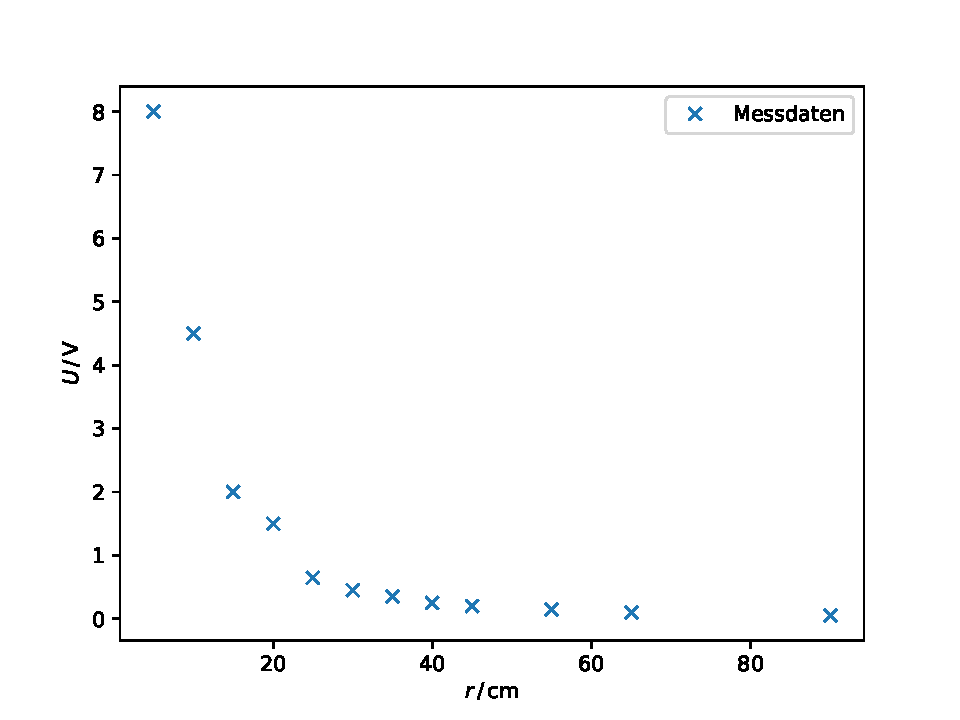
\includegraphics{build/plot_3.pdf}
  \caption{Dampfdruckkurve.}
  \label{fig:Dampfdruckkurve}
\end{figure}
\noindent Durch lineare Ausgleichsrechnung können dann die Parameter $b= \num{8.1}$ und $m= \SI{-2281.56}{\kelvin}$ bestimmt werden:
Aus dem bereits genannten Zusammenhang \eqref{eqn:ccg} ergibt sich die Verdampfungswärme $L$ nun zu
\begin{align*}
  L = -m \cdot R = \SI[per-mode=fraction]{19231 +- 572}{\joule\per\mol},
\end{align*}
wobei für $R$ der Wert \SI{8.314}{\joule\per\mol\per\kelvin} genutzt wird. \cite{codata}
Aus dem allgemeinen Zusammenhang für die Verdampfungswärme \eqref{eqn:md} kann nun der Massendurchsatz bestimmt werden:

\begin{table}
  \centering
  \caption{Massendurchsatz.}
  \label{tab:tabelle4}
  \sisetup{table-format=1.2}
  \begin{tabular}{c c c}
    \toprule
    {$t [\si{\second}]$} & {$T_2 [\si{\kelvin}]$} & {$\frac{\symup{d} m}{\symup{d} t} [\si{\mol\per\second}]$} \\
    \midrule
    \num{120}            & \num{22.8 +- 0.1}      & $(1.26 \pm 0.04) \times 10^{-6}$                           \\
    \num{240}            & \num{25.5 +- 0.1}      & $(1.26 \pm 0.05) \times 10^{-6}$                           \\
    \num{360}            & \num{28.9 +- 0.1}      & $(1.26 \pm 0.05) \times 10^{-6}$                           \\
    \num{480}            & \num{32.5 +- 0.1}      & $(1.26 \pm 0.06) \times 10^{-6}$                           \\
    \bottomrule
  \end{tabular}
\end{table}


\subsection{Kompressorleistung}
Um die Wärmemenge als Kondensationswärme an das Reservoir $R_1$ abgeben zu können, komprimiert der Kompressor $K$ das Gas, so dass es flüssig wird.
Für die mechanische Kompressorleistung $P_{\text{mech}}$ ergibt sich
\begin{equation}
  P_{\text{mech}} = \frac{1}{\kappa -1}\Bigl(p_b \sqrt[\kappa]{\frac{p_a}{p_b}} - p_a \Bigr) \frac{1}{\rho} \frac{\increment m}{\increment t} \cdot M \cdot 10^{-3}.
\end{equation}
$\kappa$ ist der Adiabatenkoeffizient des Mediums, für $\ce{Cl2F2C}$ durch $\kappa = 1.14$ gegeben \cite{sample}, $p_a$ und $p_b$ die Drücke bei denen der Kompressor arbeitet, $\rho$ die Dichte des Gases unter $p_a$, $\frac{\increment m}{\increment t}$ der Massendurchsatz und $M$ die Molmasse des Mediums, für $\ce{Cl2F2C}$ durch $M = \SI{120.91}{\gram\per\mol}$ gegeben. Der Faktor $10^{-3}$ wurde ergänzt, um den Massendurchsatz in SI-Einheiten umzurechnen. \\
Um die Dichte $\rho$ zu bestimmen, wird der Zusammenhang
\begin{equation}
  \frac{p_i}{\rho_iT_i} = \frac{p_0}{\rho_0T_0}
\end{equation}
verwendet, wobei $\rho_0 = \SI{5,51}{\gram\per\litre}$ die Dichte des Transportmediums bei $T_0 = \SI{0}{\celsius}$ und $p_0 = \SI{1}{\bar}$ ist \cite{sample}.
Umgestellt nach $\rho$ ergibt sich
\begin{equation*}
  \rho = \frac{\rho_0 \ T_0 \ p_a}{p_0 \ T_2} \ .
\end{equation*}
Hieraus können die Dichten $\rho_i$ für alle Messzeitpunkte berechnet werden.
Für den Fehler der Kompressorleistung wurde dabei die Fehlerformel
\begin{equation}
  \increment{P_{\text{mech}}} = \sqrt{\Bigl(\frac{\partial P_{\text{mech}}}{\partial p_a}\increment{p_a}\Bigr)^2 + \Bigl( \frac{\partial P_{\text{mech}}}{\partial p_b}\increment{p_b}\Bigr)^2 + \Bigl( \frac{\partial P_{\text{mech}}}{\dot{m}} \increment{\dot{m}}  \Bigr)^2}
\end{equation}
verwendet, $\dot{m}$ beschreibt hierbei den Massendurchsatz.

\begin{table}
  \centering
  \caption{Kompressorleistung.}
  \label{tab:tabelle5}
  \sisetup{table-format=1.2}
  \begin{tabular}{c c c}
    \toprule
    {$t [\si{\second}]$} & {$\rho [\si{\gram\per\litre}]$} & {$P_{\text{mech}} [\si{\joule\per\second}]$} \\
    \midrule
    \num{120}            & \num{38.1 +- 1.0}               & $(1.34 \pm 0.05) \times 10^{-4}$               \\
    \num{240}            & \num{45.3 +- 1.1}               & $(1.27 \pm 0.05) \times 10^{-4}$               \\
    \num{360}            & \num{44.7 +- 1.1}               & $(1.28 \pm 0.05) \times 10^{-4}$               \\
    \num{420}            & \num{46.7 +- 1.1}               & $(1.26 \pm 0.05) \times 10^{-4}$               \\
    \bottomrule
  \end{tabular}
\end{table}